%%%%%%%%%%%%%%%%%%%%%%%%%%%%%%%%%%%%%%%%%%%%%%%%%%%%%%%%%%%%%%%%%%%%%%%%%%%%%%%
\section{EXPERIMENTAL RESULTS}
%%%%%%%%%%%%%%%%%%%%%%%%%%%%%%%%%%%%%%%%%%%%%%%%%%%%%%%%%%%%%%%%%%%%%%%%%%%%%%%

%AS-P: 39 flights, 24 this summer
%AS-S1: 9 flights, 9 this summer
A total of 79 hours of flight testing have been performed in 46 flights with the two \textit{AtlantikSolar} UAVs designed and built at ETH Zurich so far. The following section briefly summarizes the main results required and obtained for efficient long-endurance flight and application of the platform in Search-And-Rescue missions.
 
%%%%%%%%%%%%%%%%%%%%%%%%%%%%%%%%%%%%%%%%%%%%%%%%%%%%%%%%%%%%%%%%%%%%%%%%%%%%%%%
\subsection{Subsystem Level Test Results}
%%%%%%%%%%%%%%%%%%%%%%%%%%%%%%%%%%%%%%%%%%%%%%%%%%%%%%%%%%%%%%%%%%%%%%%%%%%%%%%
 
%%%%%%%%%%%%%%%%%%%%%%%%%%%%%%%%%%%%%%
\subsubsection{Measurement of required level flight power} \label{secsec:LevelFlightPower}
%%%%%%%%%%%%%%%%%%%%%%%%%%%%%%%%%%%%%%
%[Philipp]

\begin{figure}[tb]
    \centering
     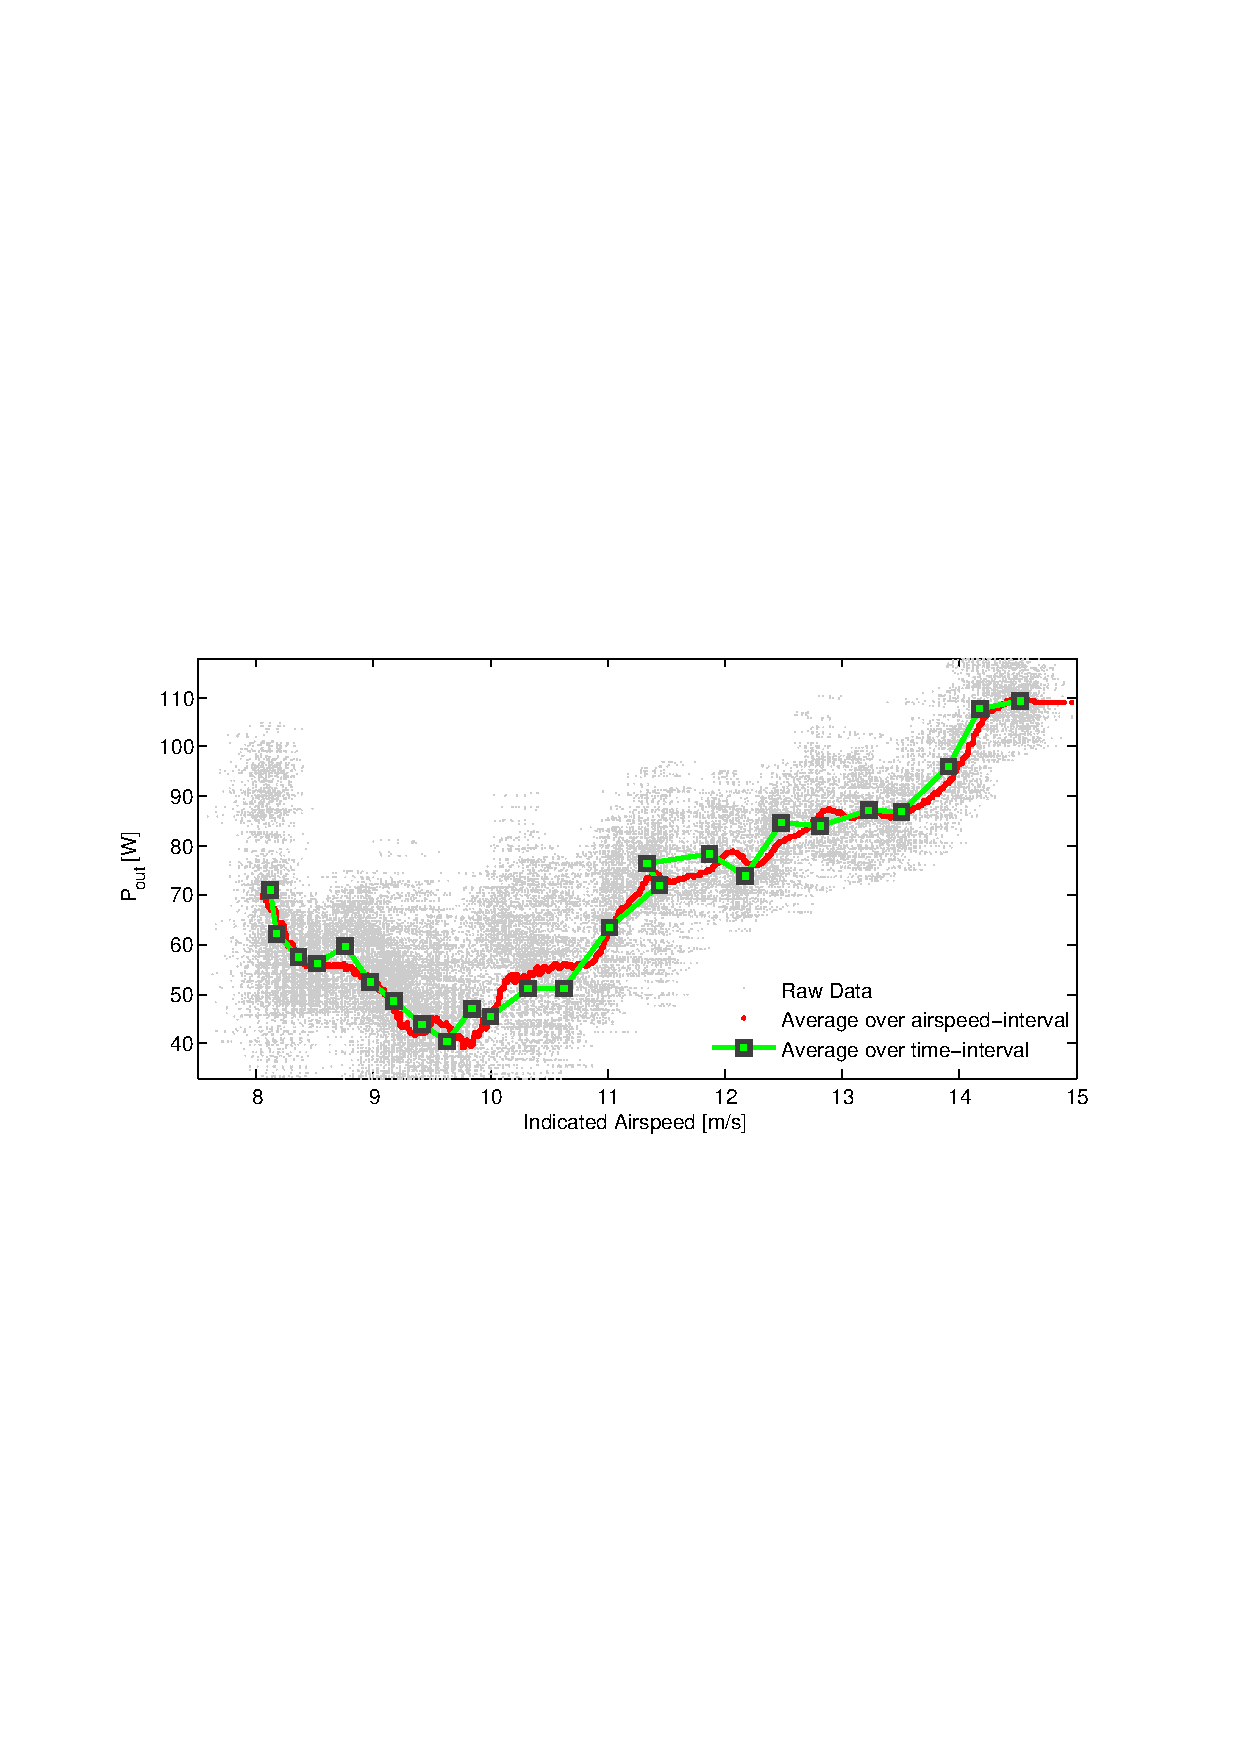
\includegraphics[width=\linewidth]{images/PowerMeasurements/PowerMeasurements}
    \caption{\textit{Power curve}, i.e. the total required level power $P_{out}$ vs. airspeed $v$, measured in constant-altitude loiter mode with $v_{ref}=const=8...15m/s$ in $T=200s$ intervals. (a) Raw data, (b) $P_{out}$ averaged over 1000 neighboring airspeed data points and (c) $P_{out}$ averaged within the $T=200s$ intervals.} 
    \label{fig:PowerMeasurements}
\end{figure}

To verify the energetic UAV modeling in Sec. \ref{sec:ConceptualDesignMethodology}, constant-altitude loitering flights performed in calm air (see Sec. \ref{sec:12hFlight}) were used to record the power curve (Figure \ref{fig:PowerMeasurements}) for \textit{AtlantikSolar}. Although a significant portion of noise remains, it can be stated that $P_{Out}^{\,min}\approx42...48W$ at $v_{air}^{\,opt}=9.7\pm0.5m/s$. The modeling through (\ref{eqn:P_out})-(\ref{eqn:C_D}) yielded $P_{out}=44.5W$ for \textit{AtlantikSolar}. This correspondance means that - on the output power side - the predicted 24h-flight capability and excess time are verified. However, it should be noted that the low power consumption from Figure \ref{fig:PowerMeasurements} was only reached after significant re-iterations on propeller, motor and motor-controller design through wind-tunnel and lab tests. In general, the modeling through (\ref{eqn:P_out})-(\ref{eqn:C_D}) is an absolute lower limit for power consumption as it assumes undisturbed flight at minimum sink airspeed, whereas in reality deviations in airspeed and attitude or even downdrafts can not be avoided.

%%%%%%%%%%%%%%%%%%%%%%%%%%%%%%%%%%%%%%
\subsubsection{Autopilot operation in challenging wind conditions}
%%%%%%%%%%%%%%%%%%%%%%%%%%%%%%%%%%%%%%    

\begin{figure}[tb]
    \centering
     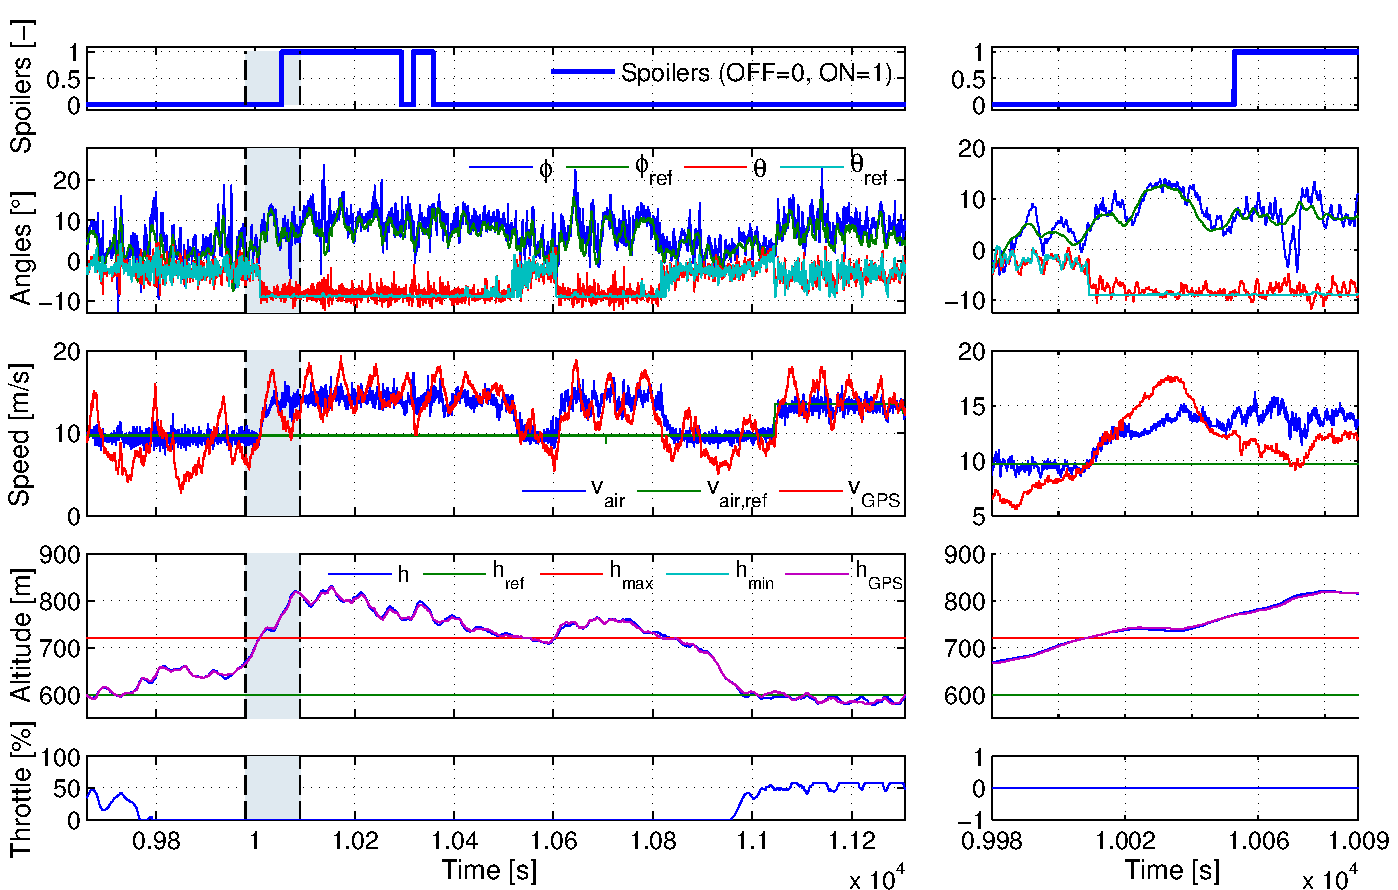
\includegraphics[width=\linewidth]{images/ControlTestFlight/ControlTestFlight.pdf}
    \caption{Fully autonomous flight in constant altitude-reference loitering mode under the influence of significant thermal updrafts and winds. Left: The autopilot engages spoilers and motor as required to respect altitude limits $h_{min}$ and $h_{max}$ in its thermal compliance mode. Right: A zoomed-in section of the left plot gives insight into attitude reference tracking.} 
    \label{fig:ControlTestFlight}
\end{figure}

Challenging wind conditions strain a UAV's state estimation and control capabilities. A segment from a fully autonomous verification flight of \textit{AtlantikSolar} under such conditions is shown in Figure \ref{fig:ControlTestFlight}. The aircraft is in constant altitude-reference loiter mode, and after hitting a thermal at $t=9760s$ it correctly switches off the motor, keeps $\theta_{ref}$ due to the implemented thermal compliance (Sec. \ref{sec:Control}) and thus gains altitude. When the altitude is above the user-prescribed $h_{max}$, negative pitch reference is prescribed and successfully tracked. The aircraft however continues to gain altitude due to the significant updraft strength. From $t=10052s$ on, the autopilot thus engages the spoilers at $h>h_{max}+50$ to achieve maximum descent rate. The aircraft's altitude begins to stabilize and the spoilers are disengaged at $t=10357s$. After a total of 20 minutes of unpowered flight, the altitude stabilizes around $h=h_{ref}$ again, with the controller now commanding high throttle due to the following downdraft. 

%%%%%%%%%%%%%%%%%%%%%%%%%%%%%%%%%%%%%%%%%%%%%%%%%%%%%%%%%%%%%%%%%%%%%%%%%%%%%%%
\subsection{Continuous 12-hour Flight} \label{sec:12hFlight}
%%%%%%%%%%%%%%%%%%%%%%%%%%%%%%%%%%%%%%%%%%%%%%%%%%%%%%%%%%%%%%%%%%%%%%%%%%%%%%%
  
%[PHILIPP]
\begin{figure}[tb]
    \centering
     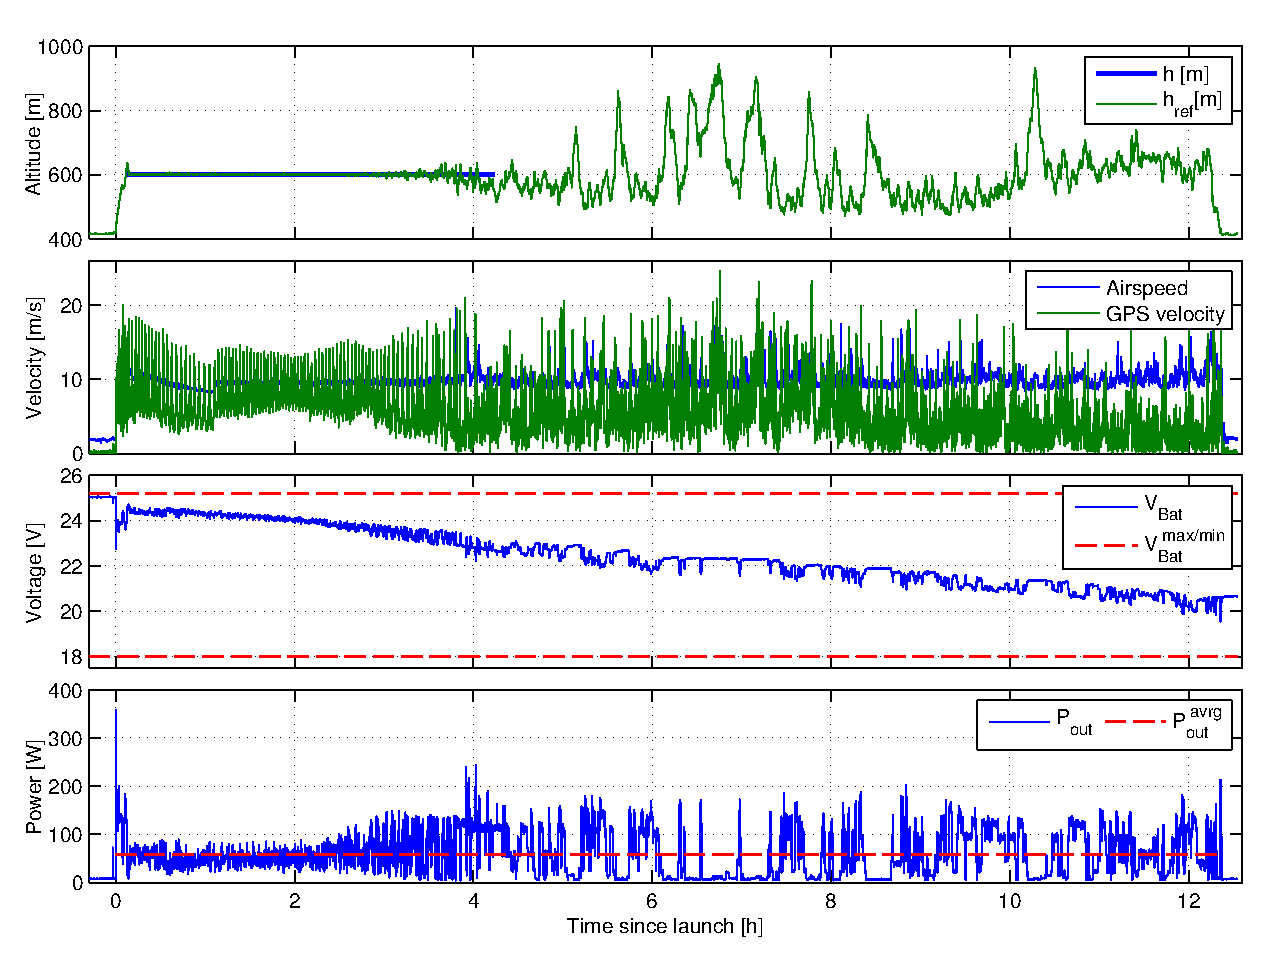
\includegraphics[width=\linewidth]{images/12hFlight}
    \caption{A 12h 22min flight performed by \textit{AtlantikSolar} to test the endurance under night-flight conditions, i.e. without solar power income. The red-dotted lines are (a) the mean of the output power (59W) over the whole flight in the power plot and (b) the battery voltage at maximum/minimum state-of-charge in the voltage plot.} 
    \label{fig:12hFlight}
\end{figure}

As a first step towards demonstrating multi-day flights, \textit{AtlantikSolar} performed a 12 hour 22 minutes (276km ground distance) flight under replicated night-conditions (Figure \ref{fig:12hFlight}), i.e. with the solar power system completely disabled. After launch at 7.15am ($t=0h$), the UAV performs autonomous constant-altitude loitering to execute the power measurements of Sec. \ref{secsec:LevelFlightPower} and switch to autopilot-assisted (SAS\&CAS) modes for additional testing at $t=4.1h$. The whole flight is marked by severe thermal down- and updrafts with altitude gains up to 350m, with the significant difference between airspeed and GPS-velocity showing horizontal winds on the order of the airspeed (up to 11m/s) for $t>4h$. Although the average power consumption of 59W is higher than determined in Sec. \ref{secsec:LevelFlightPower}, the batteries still show a remaining state of charge (SoC) of ca. 23\% (corresponding to $V_{Bat}$=20.6V) after landing. Simple extrapolation using the remaining SoC shows that flight times of $t_{endurance}=15h$ (and even more in calmer conditions) are possible solely on batteries. Crossing the night for the full operating range defined in Sec. \ref{sec:ConceptDesignApplication} and involving $t_{night}^{\,max}=10.5h$ on April 21\textsuperscript{st} thus seems possible with excess times of $t_{exc}>4.5h$. This supports the findings of the conceptual design. 

%%%%%%%%%%%%%%%%%%%%%%%%%%%%%%%%%%%%%%%%%%%%%%%%%%%%%%%%%%%%%%%%%%%%%%%%%%%%%%%
\subsection{Mapping Flights in Search and Rescue Scenarios}
%%%%%%%%%%%%%%%%%%%%%%%%%%%%%%%%%%%%%%%%%%%%%%%%%%%%%%%%%%%%%%%%%%%%%%%%%%%%%%%

%	This subsection presents some example results of the MeF ICARUS Field Testing for the AtlantikSolar System Overview paper
The AtlantikSolar is utilized within several research projects. Within that framework, it recently participated in the ICARUS project~\cite{ICARUSsite} field--trials event that took place in Marche--en--Famenne, Belgium. During these trials, several of the platform capabilities were presented and especially its autonomous long--term operation as required by the SAR teams for collecting aerial data that can be utilized for mapping purposes and capturing thermal images for victim detection. The sensor pod described in Sec.~\ref{sec:detailed_design} was used on--board recording pose--annotated visible--light grayscale and thermal images from an HDR global shutter camera (Aptina MT9V034) and a FLIR Tau2 respectively. Furthermore, a Sony HDR-AS100VW camera with GPS tagging was also carried onboard. The UAV executed several pre--planned missions ensuring the complete coverage of a given map with its sensors and, with the help of the Pix4D software~\cite{Pix4Dsite}, the pose--annotated images enabled the dense reconstruction of $3\textrm{D}$ models of the area. Figure~\ref{fig:mef_icarus_reconstruction} presents such results, the reference waypoints and their radius of acceptance along with the recorded flight path and segments of the densified point clouds. 


%
%%%%%%%%%%%%%%%%%%%%%%%%%%%%%%%%%%%%%%%%%%%%%%%%%%%%%%%%%%%%%%%%%%%%%%%%%%%%%%
\begin{figure}[htbp]
\begin{center}
  \includegraphics*[width=8.5cm]{images/MeF_GS_RGB_Merged_v4.eps} % 
\end{center}
\caption{Inspection mission reference waypoints and recorded path along with dense point clouds of sectors of the $3\textrm{D}$ reconstruction using the Aptina grayscale camera and the Sony RGB camera. The derived maps come with geoinformation while a small amount of highly--accurate ground control points (GCPs) can improve the georeferencing accuracy and also enable the seamless merging of different point clouds.  }
\label{fig:mef_icarus_reconstruction}
\end{figure}
%%%%%%%%%%%%%%%%%%%%%%%%%%%%%%%%%%%%%%%%%%%%%%%%%%%%%%%%%%%%%%%%%%%%%%%%%%%%%%
%


%[DRALEXIS]
%    - mapping missions in ICARUS. 
%    - REF to Separate paper??? Yes, but only once both are accepted.
%   - some cool pics/reconstructed maps